\subsection{RAID 5}

RAID 5 mejora la idea de RAID 4 al distribuir tanto los datos como la paridad entre todos los discos. De esta forma, elimina el cuello de botella que producía el disco de paridad dedicado.

Al igual que RAID 4, utiliza striping a nivel de bloques y almacena información de paridad para poder reconstruir los datos si un disco falla. La diferencia es que la paridad no se guarda siempre en el mismo disco, sino que rota entre todos ellos.

Por ejemplo, con tres discos (Figura \ref{fig:raid5}):
\begin{figure}[!ht]
  \centering
  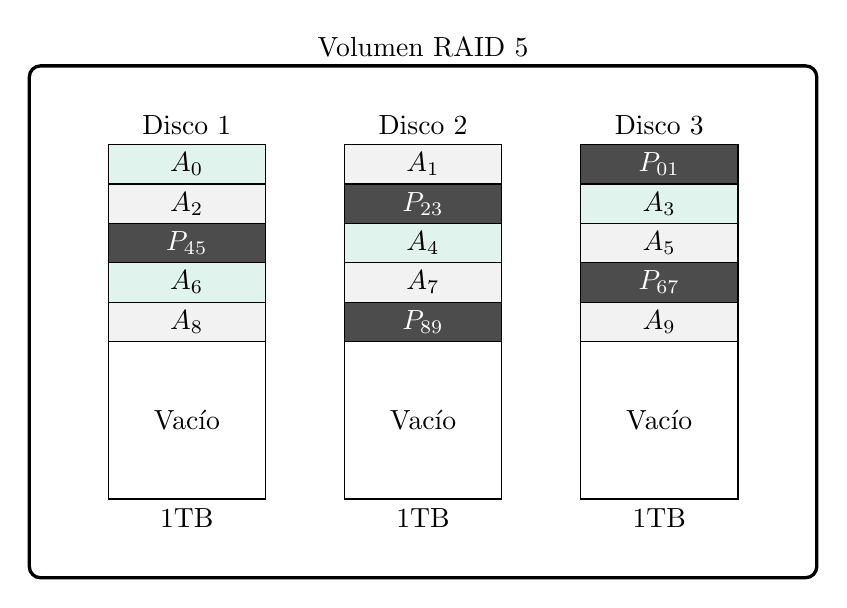
\begin{tikzpicture}
    \node[above] at (1,2.5) {Disco 1};
    \foreach \y\t\c in {
        0/A_8/gray!10,
        0.5/A_6/white!95!blue!93!green,
        1/\color{white}P_{45}/black!70,
        1.5/A_2/gray!10,
        2/A_0/white!95!blue!93!green}{
      \draw[fill=\c] (0,\y) rectangle node{\(\t\)} (2,{0.5+\y});
    }
    \draw (0,0) rectangle node{Vacío} (2,-2);
    \node[below] at (1,-2) {1TB};

    \node[above] at (4,2.5) {Disco 2};
    \foreach \y\t\c in {
        0/\color{white}P_{89}/black!70,
        0.5/A_7/gray!10,
        1/A_4/white!95!blue!93!green,
        1.5/\color{white}P_{23}/black!70,
        2/A_1/gray!10}{
      \draw[fill=\c] (3,\y) rectangle node{\(\t\)} (5,{0.5+\y});
    }
    \draw (3,0) rectangle node{Vacío} (5,-2);
    \node[below] at (4,-2) {1TB};

    \node[above] at (7,2.5) {Disco 3};
    \foreach \y\t\c in {
        0/A_9/gray!10,
        0.5/\color{white}P_{67}/black!70,
        1/A_5/gray!10,
        1.5/A_3/white!95!blue!93!green,
        2/\color{white}P_{01}/black!70}{
      \draw[fill=\c] (6,\y) rectangle node{\(\t\)} (8,{0.5+\y});
    }
    \draw (6,0) rectangle node{Vacío} (8,-2);
    \node[below] at (7,-2) {1TB};

    \draw[very thick,rounded corners] (-1,-3) rectangle (9,3.5);
    \node[above] at (4,3.5) {Volumen RAID 5};
  \end{tikzpicture}
  \caption{Tamaño del volumen de RAID 5: 2TB.}
  \label{fig:raid5}
\end{figure}
Cada fila contiene bloques de datos y un bloque de paridad, de forma similar a RAID 4, pero la paridad se almacena de forma alternada entre los discos disponibles. Al igual que RAID 4, la paridad se calcula mediante la operación XOR entre los datos.

Si falla un disco, el bloque faltante puede reconstruirse aplicando nuevamente XOR sobre los bloques restantes y la paridad.

\paragraph{Ventajas:}
\begin{itemize}
  \item Tolera la falla de un disco.
  \item No existe un único disco de paridad que limite el rendimiento o sufra mayor estrés mecánico.
  \item Excelente aprovechamiento del espacio: solo se pierde la capacidad equivalente a un disco para almacenar la paridad.
  \item Buen rendimiento en lectura.
\end{itemize}

\paragraph{Desventajas:}
\begin{itemize}
  \item Las escrituras son más lentas que en RAID 0, porque requieren recalcular y actualizar la paridad.
  \item La reconstrucción tras la falla de un disco puede ser lenta y exige mucho trabajo a los discos restantes.
\end{itemize}

\paragraph{Velocidad de Escritura}
Generalmente depende de la controladora, ya que al igual que RAID 4 requiere calcular la paridad entre los datos del Disco 1 y el Disco 2. A modo de ejemplo si se tiene \(A_0\) y se inserta \(A_1\), una escritura tendrá las siguientes cuatro operaciones:
\begin{enumerate}
  \item Escribir \(A_1\)
  \item Leer \(A_0\)
  \item Calcular \(P_{01}=A_0\oplus A_1\)
  \item Escribir \(P_{01}\)
\end{enumerate}

De este modo, si se supone la velocidad del Disco igual a 100~MB/s, resulta que 
\[
  \text{Velocidad de escritura relativa a un disco} = \frac{100~\text{MB/s}}{4} = 25~\text{MB/s}
\]

\begin{table}[!ht]
  \centering
  \begin{tabular}{l|c}
    Cantidad de discos mínima & 3 \\\hline
    Cantidad de discos que pueden fallar & 1 \\ \hline
    Velocidad de escritura relativa a un disco & \(\frac{\text{VDisco}}{\text{Cant. Oper.}}\)~[MB/s] \\\hline
    Velocidad de escritura ponderada & 2 \\ \hline
    Velocidad de lectura relativa a un disco & VDisco~[MB/s] \\ \hline
    Velocidad de lectura ponderada & 5 \\ \hline
    Costo & Medio
  \end{tabular}
  \caption{Características del RAID 5.}
\end{table}

\paragraph{Ejemplo}
Con cuatro discos de 1 TB:
\begin{itemize}
  \item Capacidad física total: 4 TB.
  \item Capacidad útil: 3 TB (la capacidad equivalente a un disco se destina a la paridad, aunque esté distribuida).
  \item Puede fallar un disco sin pérdida de datos.
\end{itemize}
